\documentclass[Lau,binding=0.6cm]{sapthesis}

\usepackage{microtype}
\usepackage[english, italian]{babel}
\usepackage[utf8]{inputenx}

\usepackage{hyperref}
\hypersetup{pdftitle={Proprietà di sicurezza nel linguaggio Rust},pdfauthor={Edoardo De Matteis}}

\usepackage{listings, float, graphicx, lipsum, cleveref, parallel, verbatim, mathtools, ebproof, comment}
\usepackage[square, sort, comma, numbers]{natbib}
\usepackage[dvipsnames]{xcolor}
\usepackage[nottoc]{tocbibind}
\usepackage[most]{tcolorbox}
\usepackage[binary-units=true]{siunitx}
\usepackage[autostyle=true]{csquotes}

% theorem box
\newtcbtheorem[number within=chapter]{Definizione}{}{
    enhanced,
    sharp corners,
    attach boxed title to top left={
        xshift=-1mm,
        yshift=-5mm,
        yshifttext=-1mm
    },
    top=1.5em,
    colback=white,
    colframe=white!50!black, %rendere solo bianco
    fonttitle=\bfseries,
    boxed title style={
        sharp corners,
        size=small,
        colback=white!50!black,
        colframe=white!50!black,
    } 
}{def}


\newtheorem{theorem}{Theorem}[section]
\newtheorem{corollary}{Corollary}[theorem]
\newtheorem{lemma}[theorem]{Lemma}

\newenvironment{myDefinition}[2]{ \begin{Definizione}[adjusted title=#1]{}{#2}
    \textbf{Definizione \thetcbcounter.} }{\end{Definizione}}

\definecolor{codegreen}{rgb}{0,0.6,0}
\definecolor{codegray}{rgb}{0.5,0.5,0.5}
\definecolor{codepurple}{rgb}{0.58,0,0.82}
\definecolor{backcolour}{rgb}{0.95,0.95,0.92}

\lstdefinelanguage{Rust}{
  keywords={},
  otherkeywords={% Operators
    0x, 0o, 0b,
    i8, i16, i32, i64, i32, i128, isize, 
    u8, i16, u32, u64, u32, u128, usize, 
    f8, f16, f32, f64, f32, f128, fsize
  },
  keywords = [2]{fn, if, in, for, let, match, struct, unsafe, while},
  keywords = [3]{as, const, move, mut},
  keywordstyle=\color{codepurple},
  keywordstyle=[2]\color{MidnightBlue},
  keywordstyle=[3]\color{Rhodamine},
  comment=[l]{//},
  morecomment=[s]{/*}{*/},
  commentstyle=\color{codegreen}\ttfamily,
  stringstyle=\color{orange}\ttfamily,
  morestring=[b]"
  }

\lstdefinestyle{mycode}{
    backgroundcolor=\color{backcolour},   
    commentstyle=\color{codegreen},
    keywordstyle=\color{MidnightBlue},
    numberstyle=\tiny\color{codegray},
    stringstyle=\color{orange},
    basicstyle=\ttfamily\footnotesize,
    breakatwhitespace=false,         
    breaklines=true,                 
    captionpos=b,                    
    keepspaces=true,                 
    numbers=left,                    
    numbersep=5pt,                  
    showspaces=false,                
    showstringspaces=false,
    showtabs=false,                  
    tabsize=2
}

\lstset{style=mycode}

% command for inline code
\newcommand{\textcode}[1]{\colorbox{backcolour}{\texttt{#1}}}

% Commands for the titlepage
\title{Proprietà di sicurezza nel linguaggio Rust}
\author{Edoardo De Matteis}
\IDnumber{1746561}
\course{Informatica}
\courseorganizer{Facoltà di Ingegneria dell'informazione, informatica e statistica}
\AcademicYear{2019/2020}
\copyyear{2020}
\advisor{Pietro Cenciarelli}
%\advisor{Dr. Nome Cognome}
%\coadvisor{Dr. Nome Cognome}
\authoremail{edoardodematteis@icloud.com}

%\examdate{16 April 2013}
%\examiner{Prof. Nome Cognome}
%\examiner{Prof. Nome Cognome}
%\examiner{Dr. Nome Cognome}
\versiondate{\today}

\begin{document}

\frontmatter

\maketitle

%\dedication{Dedicato a\\ Donald Knuth}

%\begin{abstract}
%\end{abstract}

%\begin{acknowledgments}
%\end{acknowledgments}

\tableofcontents

% Do not use the starred version of the chapter command!

\mainmatter

\chapter{Introduzione} \label{sec:politica_di_sicurezza}
Il linguaggio di programmazione C è stato sviluppato nel 1978 e ad oggi è ancora uno dei più popolari ~\cite{tiobe:index} ~\cite{pypl:index}, ciò è dovuto al fatto che circa il 98\% ~\cite{real_men_program_in_c} dei sistemi informatici sul mercato sono sistemi integrati che richiedono un basso overhead e C risponde a questa esigenza tramite una gestione manuale della memoria. 
Allo stesso tempo C permette di scrivere programmi non sicuri proprio a causa della gestione esplicita della memoria, esistono linguaggi considerati sicuri quali Java che gestiscono automaticamente la memoria tramite \textbf{garbage collection} (definizione \ref{def:garbage_collection}) al prezzo di un maggiore overhead e sono quindi poco adatti alla scrittura di codice per embedded systems.

\begin{myDefinition}{Garbage collection}{garbage_collection}
    È una delle tecniche di gestione automatica della memoria più usate nei linguaggi di programmazione: tramite un modulo noto come \textbf{garbage collector} si tiene traccia di ogni allocazione e le zone di memoria non più necessarie vengono periodicamente liberate, rendendole nuovamente disponibili. La garbage collection ha il vantaggio di esonerare il programmatore dal dover gestire la memoria così da potersi concentrare sulla logica del programma e la sua leggibilità, si evitano inoltre vulnerabilità quali double free o dangling pointer (rispettivamente sezioni \ref{sec:double_free} e \ref{sec:dangling_reference}). Con la garbage collection l'esecuzione dei programmi è però più lenta data la presenza del garbace collector.
\end{myDefinition}

Nel breve futuro ci si aspetta sempre un numero crescente di oggetti d'uso comune connessi tra loro (i.e. internet of things) e si sente la necessità di metodi sicuri per programmare sistemi integrati. Nella ricerca di un linguaggio sicuro con gestione esplicita della memoria Rust sembra essere il miglior candidato: il sistema dei tipi di Rust è detto lineare, questa scelta di sviluppo prende forma nei meccanismi di \textbf{ownership} e \textbf{borrowing} (definizioni \ref{def:ownership} e \ref{def:borrowing}) e \textbf{lifetime}. 

Nella sintassi e nella semantica di un sistema tipato (capitolo \ref{chap:type_safety}) è presente il contesto $\Gamma$ ovvero un insieme composto da coppie nella forma $x:T$ con $x$ variabile e $T$ tipo ed un operatore "$,$" che concatena due o più contesti tra loro in un nuovo contesto. Non sono ammesse ripetizioni di variabili e si assume che venga loro applicata automaticamente una ridenominazione, l'$\alpha$-regola garantisce che il contesto manterrà la sua consistenza. Consideriamo le tre seguenti proprietà base dette \textit{strutturali}:

\begin{lemma}[Exchange] \label{lemma:exchange}
  All'interno di un contesto l'ordine delle coppie è irrilevante.
  \begin{equation*}
      \Gamma_{1},x_{1}:T_{1},x_{2}:T_{2},\Gamma_{2} \vdash t:T \longrightarrow \Gamma_{1},x_{2}:T_{2},x_{1}:T_{1},\Gamma_{2} \vdash t:T
  \end{equation*}
\end{lemma}

\begin{lemma}[Weakening] \label{lemma:weakening}
  L'aggiunta nel contesto di coppie non necessarie è irrilevante ai fini del calcolo dei sequenti.
  \begin{equation*}
      \Gamma_{1},\Gamma_{2} \vdash t:T \longrightarrow \Gamma_{1},x_{1}:T_{1},\Gamma_{2} \vdash t:T
  \end{equation*}
\end{lemma}

\begin{lemma}[Contraction] \label{lemma:contraction}
  Se abbiamo una derivazione con due assunzioni identiche allora possiamo avere lo stesso risultato usandone una sola.
  \begin{equation*}
      \Gamma_{1},x_{2}:T_{1},x_{3}:T_{1},\Gamma_{2} \vdash t:T_{2} \longrightarrow \Gamma_{1},x_{1}:T_{1},\Gamma_{2} \vdash \sigma(t):T
  \end{equation*}
  Sia $\sigma$ la sostituzione $\{ x_{2} \mapsto x_{1}, x_{3} \mapsto x_{1} \}$.
\end{lemma}

Una logica è detta \textit{substrutturale} quando almeno una delle seguenti proprietà è omessa e se ad essere omesse sono sia weakening che contraction si parla di logica lineare ~\cite{girard:linear_logic} e, contrariamente alle logiche tradizionali nelle quali si ha a che fare con la verità di proposizioni, le logiche lineari trattano la disponibilità di risorse. Tony Hoare nel 1987 pose questo esempio: supponiamo di rappresentare in logica del primo ordine con la proposizione \textit{candy} il fatto di avere una caramella e con la proposizione \textit{\$1} il possesso di un dollaro, per esprimere l'atto di compravendita di una caramella possiamo scrivere $ \textit{\$1} \rightarrow \textit{candy} $.

\begin{equation*}
  \begin{prooftree}
    \hypo{\textit{\$1} \rightarrow \textit{candy}}
    \hypo{\textit{\$1}}
    \infer2[modus ponens]{\textit{candy}}
  \end{prooftree}
\end{equation*}

Se ne deduce $ \textit{\$1} \land \textit{candy} $ e si ha una caramella senza aver pagato, si può evitare questo problema con modellazioni differenti della base di conoscenza ma si incorre nel \textit{frame problem} \footnote{In intelligenza artificiale è il problema di dover rappresentare una conoscenza in logica senza ricorrere a numerosi assiomi i quali indicano solo che l'ambiente non cambia arbitrariamente.}. 

Un sistema lineare ~\cite{walker:linear_logic}, basato quindi su logica lineare, permettendo exchange ma non weakening né contraction garantisce che ogni variabile venga usata al più una volta, a tal fine nella sintassi di una logica lineare sono presenti dei qualificatori che indicano se la variabile marcata possa essere usata solo una volta o meno, in Rust ad esempio sui tipi primitivi non è posta alcuna restrizione. 

Per garantire la non riusabilità di una variabile vengono imposte due invarianti:

\begin{enumerate}
    \item Le variabili lineari sono usate esattamente una volta per ogni cammino nel diagramma di flusso.
    \item Espressioni unrestricted non possono contenere espressioni lineari; in generale espressioni meno restrittive non possono contenere espressioni più restrittive. 
\end{enumerate}

Il perché la prima invariante sia fondamentale è chiaro, per la seconda supponiamo di avere un oggetto \texttt{X} unrestricted con un attributo \texttt{X.y} lineare, sarebbe possibile sfruttare la permissività di \texttt{X} per usare più volte \texttt{X.y}, si avrebbe in questo una violazione della linearità.

\begin{myDefinition}{Ownership}{ownership}
    L'ownership rappresenta il possesso di un right value da parte di un left value (rispettivamente l'insieme delle espressioni che compaiono a destra e sinistra di un assegnamento). Al momento dell'inizializzazione di un oggetto di tipo non primitivo la sua variabile, se presente, è l'unico owner e con un assegnamento ad una seconda variabile la prima perde di validità. Un owner viene invalidato quando il suo scope termina, bisogna porre particolare attenzione in questo caso dato che le chiamate di funzioni possono invalidare una variabile passatavi come argomento: l'ownership è passata alla nuova variabile nel corpo della funzione e una volta terminato il suo scope non sarà più possibile accedere all'oggetto. 

    \lstinputlisting[language=Rust,caption={Ownership}, label={lst:ownership}]{../code/Ownership/own.rs}
\end{myDefinition}

\begin{myDefinition}{Borrowing}{borrowing}
  L'ownership è fondamentale per garantire una gestione automatica e sicura della memoria senza garbage collector ma non è sempre desiderabile prendere possesso di un oggetto, in questi casi si ricorre al borrowing tramite il quale si possono creare molteplici  riferimenti ~\cite[4.2]{rust:language} ad un dato purché in sola lettura, tramite il modificatore \textcode{mut} si può creare un riferimento modificabile a patto che in qualsiasi momento per ogni variabile se ne abbia al più uno. Un modulo chiamato \textbf{borrow checker} garantisce a tempo di compilazione che finché esistono dei riferimenti ad un oggetto l'oggetto stesso non possa essere distrutto. 

    \lstinputlisting[language=Rust,caption={Borrowing}, label={lst:borrowing}]{../code/Borrowing/borr.rs}
\end{myDefinition}

Un lifetime è un costrutto che il borrow checker usa per garantire che ogni riferimento sia valido, il lifetime di una variabile inizia quando viene creata e termina quando viene distrutta, quando possibile il compilatore inferisce i lifetime e in caso contrario è necessario gestirli manualmente. È paragonabile allo scope di una variabile ma non sono esattamente la stessa cosa, nel listato \ref{lst:lifetime} si può notare come le variabili \textcode{x} e \textcode{y} abbiano due scope differenti ma lo stesso lifetime \textcode{\textquotesingle a}.
  
\lstinputlisting[language=Rust]{../code/Lifetime/life.rs}
\lstinputlisting[caption={Lifetime e scope}, label={lst:lifetime}]{../code/Lifetime/output/life.txt}

Si parla di \textbf{outliving} quando per una variabile è possibile mantenere il riferimento ad un'altra variabile fuori dal suo scope. Nell'ownership (listato \ref{lst:lifetime_ownership}) chiaramente non ci sono problemi perché il possesso viene semplicemente trasferito, nel borrowing invece interviene il borrow checker (listato \ref{lst:lifetime_borrowing})

\lstinputlisting[language=Rust]{../code/Lifetime/life_own.rs}
\lstinputlisting[caption={Lifetime e ownership}, label={lst:lifetime_ownership}]{../code/Lifetime/output/life_own.txt}

\lstinputlisting[language=Rust]{../code/Lifetime/life_bor.rs}
\lstinputlisting[caption={Outliving, il borrow checker interviene.}, label={lst:lifetime_borrowing}]{../code/Lifetime/output/life_bor.txt}

Si può eludere il controllo dell'outliving del borrow checker cambiando il tipo di \textcode{y} da \textcode{i32} a \textcode{\&i32} (listato \ref{lst:lifetime_borrowing_allowed}) purché il dato in questione sia di tipo primitivo e non composto (listato \ref{lst:lifetime_borrowing_temporary}). 

Una \textbf{temporary} è una variabile anonima inizializzata con il risultato di un'espressione, verrà usata per le successive valutazioni e perderà validità solo al termine del suo scope come qualsiasi variabile. A \textcode{Box::new(12)} corrisponde una temporary e quando si tenta di leggerne il valore fuori dal suo scope il compilatore segnala l'errore. Questo problema non si presenta con i tipi primitivi perché evidentemente Rust esegue delle \textbf{deep copy}, si ha infatti un comportamento simile più all'ownership che al borrowing. 

\lstinputlisting[language=Rust]{../code/Lifetime/life_bor_allowed.rs}
\lstinputlisting[caption={Lifetime e borrowing tipi primitivi.}, label={lst:lifetime_borrowing_allowed}]{../code/Lifetime/output/life_bor_allowed.txt}

\lstinputlisting[language=Rust]{../code/Lifetime/life_temp.rs}
\lstinputlisting[caption={Lifetime e borrowing tipi composti.}, label={lst:lifetime_borrowing_temporary}]{../code/Lifetime/output/life_temp.txt}

Quando a seguito di un assegnamento la variabile memorizza un riferimento ad un oggetto si parla di \textbf{shallow copy}, se invece si memorizza il dato per intero si ha una una \textbf{deep copy}. 
In Rust per i dati di tipo primitivo si eseguono sempre deep copy mentre per gli oggetti composti si eseguono di default shallow copy, è comunque possibile copiare l'oggetto nella sua interezza tramite il \textbf{trait} (simile a quello che in Java è un'interfaccia) \textcode{Clone}; questo avviene poiché di un dato di tipo primitivo la dimensione è nota a tempo di compilazione e non si può dire lo stesso degli oggetti composti. Nel listato \ref{lst:ownership_primitive} \textcode{x} e \textcode{y} puntano a due locazioni differenti.

\lstinputlisting[language=Rust, caption={Ownership con tipi primitivi.}, label={lst:ownership_primitive}]{../code/Ownership/own_prim.rs}

I controlli su ownership e borrowing sono eseguiti a tempo di compilazione rendendo l'esecuzione molto più rapida e sicura, questi vantaggi si ottengono al prezzo di un linguaggio più verboso e che richiede maggior impegno cognitivo da parte del programmatore. 


\chapter{Security policy}

Risulta molto difficile parlare di sicurezza in generale dato che non ne esiste una definizione assoluta ma è un concetto relativo che varia in base a cosa ci interessa proteggere e garantire. La sicurezza di un'organizzazione - che essa sia una multinazionale o un singolo individuo - è definita da una \textbf{security policy}  ovvero un documento contenente regole, principi e pratiche che determinano come garantire che il sistema si trovi in uno stato sicuro ~\cite{milner:type_polymorphism}. 

\begin{myDefinition}{Security policy}{security_policy}
    In una politica di sicurezza si definiscono quali azioni i \textbf{principal} possono eseguire sugli oggetti. Un principal è un'entità qualsiasi che interagisce con il sistema e deve rispettare la politica di sicurezza, nel caso specifico dei linguaggi di programmazione saranno entità software.
\end{myDefinition}

Nello sviluppo di linguaggi di programmazione sicuri si è guidati da due principi ~\cite{nino:security_programming_language}:
\begin{itemize}
    \item \textbf{Trusted computing base (TCB)}. Un sistema presenta componenti critici per il rispetto della policy, questi formano il TCB ed è fondamentale non presenti vulnerabilità dato che metterebbero a repentaglio la sicurezza del sistema stesso, il TCB deve essere semplice e limitato così da poterne verificare facilmente la correttezza ed evitare fallimenti. 
    \item \textbf{Principle of Least Privilege (POLP)}. Durante l'esecuzione ogni entità deve avere il numero minore possibile di permessi necessari per eseguire il suo compito. 
\end{itemize} 
È possibile scomporre i requisiti di sicurezza fondamentali durante lo sviluppo in \textbf{access control} e \textbf{information flow}, il primo limita chi o cosa possa accedere a quali risorse e il secondo definisce quali operazioni siano corrette o meno in seguito ad un accesso conforme all'accesso control, di norma il sistema operativo stesso implementa questi controlli via software o hardware e programmi che sono legali in C potrebbero non esserlo per l'OS. 
In Rust la sicurezza è garantita da regole semplici e verificabili e si rispetta il POLP, i controlli sono eseguiti a tempo di compilazione e anche quando un programma viene interrotto a runtime non non viene scomodato il sistema operativo (vedere ad esempio il codice nel listato \ref{lst:integeroverflowrs}).

Questa necessità di implementare la sicurezza nel linguaggio stesso e non rimetterla più nelle mani del sistema operativo è nata dall'avvento di internet e la sempre più grande condivisione di codice potenzialmente pericoloso.

Per dimostrare delle proprietà di un linguaggio serve una definizione formale della sua \textbf{semantica} ovvero l'insieme delle regole che definiscono il significato di un linguaggio e dei suoi programmi.
A tal proposito Rust non ha una semantica formale (figura \ref{fig:warning}) e la sua definizione di sicurezza è poco chiara, un programma è sicuro se rispetta \textbf{memory safety} (capitolo \ref{chap:memory_safety}) e \textbf{semantica statica} (capitolo \ref{chap:type_safety}) ~\cite[14]{rust:reference} ma la documentazione presenta delle definizioni poco chiare se non addirittura contraddittorie: 

\vspace{5mm}

\begin{Parallel}{0.48\textwidth}{0.48\textwidth}
    \selectlanguage{english}
    \ParallelLText{
        "Rust code is incorrect if it exhibits any of the behaviors in the following list. This includes code within \colorbox{backcolour}{\texttt{unsafe}} blocks and \colorbox{backcolour}{\texttt{unsafe}} functions. \colorbox{backcolour}{\texttt{unsafe}} only means that avoiding undefined behavior is on the programmer; it does not change anything about the fact that Rust programs must never cause undefined behavior." ~\cite[14.3]{rust:reference}
    }
    
    \selectlanguage{italian}
    \ParallelRText{
        "Del codice in Rust non è corretto se presenta almeno uno dei comportamenti in lista. Questo vale anche per codice in blocchi \colorbox{backcolour}{\texttt{unsafe}} e funzioni \colorbox{backcolour}{\texttt{unsafe}}. \colorbox{backcolour}{\texttt{unsafe}} significa solo che evitare undefined behaviour è compito del programmatore; non cambia alcuna garanzia sul fatto che i programmi in Rust non debbano mai causare undefined behaviour." 
    }
    \ParallelPar
\end{Parallel}

\vspace{5mm}

L'uso del termine "unsafe" è causa di confusione dal momento che \colorbox{backcolour}{\texttt{unsafe}} è un costrutto sintattico che consente la scrittura di codice che può causare \textbf{undefined behavior}, per questo si dice che Rust è composto da due "sottolinguaggi": \textit{unsafe Rust} e \textit{safe Rust} in base alla presenza o meno di un blocco \colorbox{backcolour}{\texttt{unsafe}} nel codice, questo costrutto è desiderabile perché permette sia di poter comunicare con librerie in \textit{C} che di avere un accesso più esplicito alla memoria ~\cite[1.2]{rust:rustonomicon}; piuttosto che una definizione formale di undefined behavior si ha una lista in continuo aggiornamento ~\cite[14.3]{rust:reference}.

Nella citazione riportata sono presenti fonti di confusione: nella stessa frase viene detto prima che in un blocco \colorbox{backcolour}{\texttt{unsafe}} sia compito del programmatore evitare undefined behavior e subito dopo viene affermato come le garanzie sulla safety siano le stesse di safe Rust, quindi anche l'assenza di undefined behavior. Volendo comunque considerare solo l'ultima affermazione, l'esecuzione in un blocco \colorbox{backcolour}{\texttt{unsafe}} di uno degli esempi in lista non dovrebbe causare undefined behavior; nel listato \ref{lst:unsafe_raw} si ha un \textbf{raw pointer dereferencing} (presente in lista come dimostrato in figura \ref{fig:warning}): è possibile leggere il valore memorizzato in una locazione di memoria tramite il suo indirizzo come in C.

È ragionevole che questo sia possibile solo in unsafe Rust ma mette in luce come la documentazione sia poco chiara. 

\lstinputlisting[language=Rust]{../code/Unsafe/raw.rs}
\lstinputlisting[caption={Raw pointer dereferencing in un blocco \texttt{unsafe}}, label={lst:unsafe_raw}]{../code/Unsafe/output/rawrs.txt}

\begin{figure}[h!t]
    \centering
    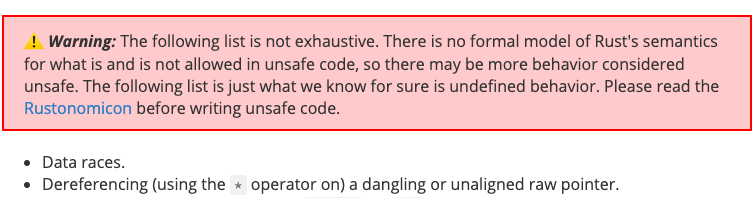
\includegraphics[scale=0.52]{images/warning_undefined_behavior.png}
    \caption{Il raw pointer dereferencing è considerato undefined behavior}
    \label{fig:warning}
\end{figure}


\chapter{Memory Safety} \label{chap:memory_safety}

Durante l'esecuzione di un programma ogni oggetto ha associato un insieme finito di locazioni di memoria cui accedere noto come \textbf{address space}, se in un programma nessun oggetto accede mai ad indirizzi fuori dal proprio address space allora è \textbf{memory safe} e un linguaggio che garantisce la memory safety dei suoi programmi è detto a sua volta memory safe.

L'address space può essere definito a tempo di compilazione o esecuzione dipendentemente dal tipo di allocazione, in C e Rust ne consideriamo tre tipi:

\begin{itemize}
    \item \textbf{Allocazione statica}. Il compilatore memorizza solo ed esclusivamente le variabili globali ovvero quelle il cui scope corrisponde a tutto il file, si possono definire tramite un modificatore (in C è \colorbox{backcolour}{\texttt{static}}, da cui il nome) o definendole fuori da ogni funzione.  
    \item \textbf{Allocazione automatica}. Si usa per variabili locali e di tipo primitivo. Una variabile è locale quando dichiarata all'interno di una funzione (quindi valida solo in un determinato scope), dal momento che l'ordine di esecuzione non è noto a tempo di compilazione l'allocazione avviene a tempo di esecuzione e si utilizza una struttura dati nota come \textbf{stack} o \textbf{call stack}. Spesso il nome call stack viene utilizzato per le sole chiamate di funzione. 
    \item \textbf{Allocazione dinamica}. L'allocazione dinamica in C è esplicita tramite funzioni come \colorbox{backcolour}{\texttt{malloc}} e permette di allocare memoria ad un oggetto durante l'esecuzione il che si rivela molto utile per oggetti che non hanno una dimensione fissa. In safe Rust non si hanno funzioni come in C per questioni di sicurezza, si ha però un tipo \colorbox{backcolour}{\texttt{Box}}, si usa una struttura dati chiamata \textbf{heap} che ha la particolarità di crescere verso l'alto contrariamente allo stack che cresce verso il basso e può essere problematico in caso di overflow (sezione \ref{sec:buffer_overflow}). Un tipo composto è definito dall'unione di tipi primitivi e non è banale prevedere la dimensione di un oggetto composto quindi vengono allocati sull'heap. Un oggetto di tipo primitivo viene salvato sullo stack. 
\end{itemize}

Questo approccio è stato reso popolare dal C ed è oggi adottato da numerosi linguaggi, sempre in C esiste un ulteriore tipo di allocazione della memoria noto come \textbf{register allocation} che permette di scrivere direttamente su un blocco del processore, non essendo presente in Rust non viene approfondita.

\section{Buffer Overflow} \label{sec:buffer_overflow}
Un \textbf{buffer} è una qualsiasi zona contigua di memoria contenente istanze dello stesso dato e ne definisce i limiti, se durante l'esecuzione si riescono a superare si parla di \textbf{buffer overflow} ed è possibile leggere o scrivere oltre il proprio address space. Un esempio di buffer overflow in C è nel listato \ref{lst:stackoverflowc} ~\cite[7.5]{stallings:os}: dato che gli array sono posizionati uno dopo l'altro (in ordine LIFO essendo dati allocati su uno stack) si riesce a leggere e scrivere su \texttt{str1} eludendo anche il controllo di uguaglianza, nel terzo caso questo controllo viene superato perché si confrontano solo i primi 8 caratteri. In Rust questo non è possibile, si veda nel listato \ref{lst:bufofrs} come il linguaggio esegua dei controlli sulle dimensioni degli array, esattamente ciò che la funzione \texttt{gets} non fa. 

\lstinputlisting[language=C]{../code/BufferOverflow/StackOverflow/StackAttack/stackattack.c}
\lstinputlisting[caption={Buffer overflow in C}, label={lst:stackoverflowc}]{../code/BufferOverflow/StackOverflow/StackAttack/output/stackattack_c.txt}

\lstinputlisting[language=Rust]{../code/BufferOverflow/bufof.rs}
\lstinputlisting[caption=Buffer overflow in Rust, label={lst:bufofrs}]{../code/BufferOverflow/output/bufof_rs.txt}

La pericolosità del buffer overflow è dovuta alla possibilità di eseguire codice arbitrario ovvero \textbf{code injection}, nel listato \ref{lst:injection} se ne ha un esempio molto semplice, per la stringa in input non si ha alcun tipo di bound check ed è possibile scrivere un comando che verrà eseguito da \colorbox{backcolour}{\texttt{system()}} con gli stessi permessi con cui si esegue il file. 

\lstinputlisting[language=C]{../code/Injection/inj.c}
\lstinputlisting[caption={Code injection in C}, label={lst:injection}]{../code/Injection/output/inj.txt}

Esistono code injection più sofisticati che sfruttando le istruzioni in assembly di un programma possono eseguire codice arbitrario sfruttando la rappresentazione in memoria di un processo ~\cite{stack_smashing_ffp}, questo è costituito da tre regioni:

\begin{itemize}
    \item \textbf{Text}. Contiene le istruzioni da eseguire e dati in sola lettura, quest'area è read-only quindi un tentativo di scrittura è intercettato dal sistema operativo. 
    \item \textbf{Data}. Contiene dati inizializzati o meno con scope globale, è in quest'area che vengono salvati i dati quando si esegue un'allocazione statica.
    \item \textbf{Stack}. Lo stack sul quale si salvano i dati con allocazione automatica. Proprio grazie allo stack si può sfruttare un buffer overflow per puntare ad un processo differente ed eseguire codice non desiderato.
\end{itemize}

%%%%%%%%%%%%%%%
\begin{comment}
\section{Stack Overflow}
Quando si chiama una funzione si salva lo \textbf{stack frame} (noto anche come \textbf{activation record} è una zona del call stack contenente dati necessari alla funzione attualmente in esecuzione) e può capitare che chiamate ricorsive facciano entrare il programma in uno stato di non terminazione, Rust individua a tempo di compilazione la ricorsione infinita e segnala l'overflow a tempo di esecuzione. In C l'errore che si vede è dato dal sistema operativo (macOS Catalina 10.15.3) perché con questa ricorsione infinita si prova ad accedere ad un frammento di memoria protetto.

\lstinputlisting[language=C]{../code/BufferOverflow/StackOverflow/Recursion/recursion.c}
\lstinputlisting[caption={Stack overflow ricorsivo in C}, label={lst:recursionc}]{../code/BufferOverflow/StackOverflow/Recursion/output/recursion_c.txt}

\lstinputlisting[language=Rust]{../code/BufferOverflow/StackOverflow/Recursion/recursion.rs}
\lstinputlisting[caption={Stack overflow ricorsivo in Rust}, label={lst:recursionrs}]{../code/BufferOverflow/StackOverflow/Recursion/output/recursion_rs.txt}
\end{comment}
%%%%%%%%%%%%%

\section{Integer Overflow} \label{sec:integer_overflow}
In qualsiasi macchina non astratta si ha memoria finita ed è rappresentabile solo un insieme finito di numeri, quando un valore è troppo grande (o piccolo) per essere rappresentato si ha un overflow. Sono due gli approcci principali per risolvere un integer overflow, ognuno basato su un'aritmetica differente:
\begin{itemize}
    \item \textbf{Modular arithmetic}. Si applica un wrapping ad ogni numero in overflow, dato il valore $n$ e una memoria a $m$ bit si memorizza $w = n \mod m$.
    \item \textbf{Saturation arithmetic}. Si applica un clamp ovvero dati $min$ e $max$ - rispettivamente il numero più grande e più piccolo rappresentabile - e un numero $n$ in memoria viene salvato
    \begin{equation*}
        c = \begin{cases}
            max & n > max \\
            min & n < min \\
            n  & \text{altrimenti} \\
        \end{cases}
    \end{equation*}
\end{itemize}

L'integer overflow ha in passato causato problemi molto seri: durante il volo inaugurale del lanciatore \textit{Ariane 5} un integer overflow dovuto ad una conversione in intero a 16 bit di un float a 64 bit ha causato una reazione a catena per cui il razzo ha virato orizzontalmente distruggendosi poco dopo il lancio, il codice scritto in Ada non prevedeva controlli di overflow come esplicitamente richiesto dai progettisti per motivi di efficienza. In Rust si hanno due modalità di compilazione: in \textbf{debug mode} si eseguono dei controlli in più rispetto alla \textbf{release mode} tra cui controlli dinamici per l'integer overflow - listato \ref{lst:integeroverflowrs} - contrariamente al C che applica direttamente wrapping.

Differenti linguaggi adottano differenti approcci: se si può prevedere il valore massimo possibile in un programma allora è in generale facile evitare integer overflow; in caso contrario si possono utilizzare metodi dinamici come in Rust. 

\lstinputlisting[language=Rust]{../code/IntegerOverflow/intof.rs}
\lstinputlisting[caption={Integer overflow in Rust}, label={lst:integeroverflowrs}]{../code/IntegerOverflow/output/intof_rs.txt}

Nel listato \ref{lst:integeroverflowc} si prende un intero come primo argomento e una stringa - idealmente di lunghezza pari al primo argomento - come secondo. Il problema sorge nella conversione da integer a short, inserendo come primo argomento 65536 ($2^{16}$ che non è rappresentabile con i soli 16 bit di uno short) si causa un buffer overflow, combinandone la pericolosità con la difficoltà di rivelamento dell'integer overflow.

\lstinputlisting[language=C]{../code/IntegerOverflow/width1.c}
\lstinputlisting[caption={Integer overflow in C}, label={lst:integeroverflowc}]{../code/IntegerOverflow/output/width1_c.txt}

\section{Double-Free} \label{sec:double_free}
Si ha un double free error ~\cite[10.4.4]{gollmann:computersecurity} quando si prova a liberare più volte la stessa zona di memoria e in Rust non è possibile grazie all'ownership, nel listato \ref{lst:doublefree_rs} si può vedere come \texttt{s1} perda validità dopo aver trasferito a \texttt{s2} il possesso della stringa cui puntava.

\lstinputlisting[language=Rust]{../code/DoubleFree/doublefree.rs}
\lstinputlisting[caption={Double free in Rust}, label={lst:doublefree_rs}]{../code/DoubleFree/output/doublefree_rs.txt}

In C invece si può osservare il codice nel listato \ref{lst:doublefree_c}: si immagini di avere un servizio ad iscrizione salvando ogni utente tramite una struct \texttt{User}: Guido libera la propria memoria che, disponibile, potrà memorizzare \texttt{Luisa} che si è appena iscritta. Il puntatore \texttt{Guido} però ora punta all'account di Luisa e con \texttt{free(Guido)} proprio l'account di Luisa viene eliminato con il risultato che non solo Luisa non ha più un account ma a quello di Carla possono accedere sia Guido che Luisa.

\lstinputlisting[language=C]{../code/DoubleFree/doublefree.c}
\lstinputlisting[caption={Double free in C}, label={lst:doublefree_c}]{../code/DoubleFree/output/doublefree_c.txt}

Il puntatore \texttt{Guido} è anche un \textbf{dangling pointer} (sezione \ref{sec:dangling_reference}).

\section{Dangling References} \label{sec:dangling_reference}
Quando un oggetto viene eliminato ma il suo puntatore no si ha un dangling pointer che permettere di accedere a memoria cui non si dovrebbe.

Immaginiamo ora che per vendicarsi Luisa abbia scritto un semplice sistema di messaggistica per leggere la corrispondenza di Guido, la procedura \texttt{send\_message} crea un puntatore di tipo \texttt{Message} che ha scope solo ed esclusivamente dentro \texttt{send\_message} ma facendo riferimento esplicito a quella locazione Luisa riesce a leggere il messaggio di Guido anche dopo che questo non esiste più. Nel listato \ref{lst:dangrefc} l'indirizzo viene stampato a schermo e inserito dall'utente (indicato da "$>$") per semplicità.

\lstinputlisting[language=C]{../code/DanglingReference/dangref.c}
\lstinputlisting[caption={Dangling pointer in C}, label={lst:dangrefc}]{../code/DanglingReference/output/dangref_c.txt}

In Rust non possiamo usare i puntatori perché l'ownership ci obbliga ad avere un puntatore solo e una volta disabilitato non possiamo più accedere a quell'area di memoria né si può leggere la locazione perché non è permesso il raw dereferencing; possiamo usare però le reference, nel listato \ref{lst:dangrefrs} \colorbox{backcolour}{\texttt{s1}} è una shallow copy di \texttt{s2}, la prima però sopravvive alla seconda e il borrow checker interviene, non è possibile quindi avere dangling reference.

\lstinputlisting[language=Rust]{../code/DanglingReference/dangref.rs}
\lstinputlisting[caption={Dangling reference in Rust}, label={lst:dangrefrs}]{../code/DanglingReference/output/dangref_rs.txt}


\chapter{Type Safety} \label{chap:type_safety}
Ogni oggetto in matematica ha un \textbf{tipo}, basti pensare al fatto che non è possibile eseguire un'operazione come $ \{13\} \land 10 $ dato che $\{13\}$ è un insieme, $10$ è un numero e $\land$ è un connettivo logico. 
In informatica un tipo è un vincolo che definisce un insieme definito di valori validi per una risorsa di un programma, in un linguaggio tipato l'insieme delle regole che assegna un tipo ad ogni espressione è detto semantica statica o \textbf{sistema dei tipi} ed è composto da quattro aspetti: \textbf{type safety}, \textbf{type casting}, \textbf{type initialization} e \textbf{immutability} ~\cite{security_framework}.

Durante l'esecuzione di un programma si può incorrere in due tipi di errore: \textbf{trapped} e \textbf{untrapped}, i primi sono facilmente riconoscibili dato che interrompono l'esecuzione del programma, i secondi no e per questo sono molto più difficili da individuare. Un linguaggio in cui nessun programma ben tipato (definizione \ref{def:type_checking}) genera errori trapped né untrapped si dice \textbf{sound}, se ne genera solo \textbf{untrapped} invece è \textbf{safe}, un linguaggio sound quindi è necessariamente type safe ~\cite{cencia:dispense}. Una definizione analoga ma meno formale di Milner spesso adottata è la seguente. 

\begin{center}
   \textit{well-typed programs cannot “go wrong”} ~\cite{milner:type_polymorphism}
\end{center}

con programmi che "vanno male" si possono intendere programmi non sound o che generano undefined behavior (sezione \ref{sec:politica_di_sicurezza}).

\begin{myDefinition}{Type checking}{type_checking}
    La fase di verifica dei vincoli imposti dai tipi può avvenire a tempo di compilazione o a tempo di esecuzione e si parla rispettivamente di type checking statico/forte e dinamico/debole. Ad un controllo statico consegue un'ottimizzazione e per questo è desiderabile ma purtroppo non è sempre possibile verificare la correttezza di un programma a tempo di compilazione e di norma sono utilizzati sia static che dynamic type checker, in Java ad esempio i controlli sui metodi sono eseguiti dinamicamente.

    Un programma che supera la fase di type checking è ben tipato.     
\end{myDefinition}
 
\section{Type casting}
Quando si esegue un'operazione tra oggetti di tipo differente può rivelarsi necessaria una conversione di tipo (type casting) e può essere esplicita o implicita, nel secondo caso si parla di \textbf{coercion}. Tipicamente i linguaggi con type checking forte eseguono pochi casting impliciti e quelli con type checking dinamico molti, Rust è fortemente tipato e non c'è coercion invece in C che è debolmente tipato sì.   

\lstinputlisting[language=C]{../code/TypeConversion/coercion.c}
\lstinputlisting[caption={Casting implicito in C}, label={lst:coercionc}]{../code/TypeConversion/output/coercion_c}

\lstinputlisting[language=Rust]{../code/TypeConversion/coercion.rs}
\lstinputlisting[caption={Casting in Rust}, label={lst:coercionrs}]{../code/TypeConversion/output/coercion_rs}

Rust non ha casting implicito perché può portare a vulnerabilità, un esempio di questa vulnerabilità è un bug del 2002 nel sistema operativo FreeBSD per cui in alcune chiamate di sistema si assumeva a priori che il valore in input fosse un intero positivo nonostante nella definizione della funzione il tipo fosse \texttt{int}. I programmatori data l'assunzione fatta non gestivano  il caso di un intero negativo tramite boundary check, questo valore veniva poi passato a \colorbox{backcolour}{\texttt{memcpy()}} che prende un \texttt{unsigned int} e a causa della coercion un valore come $-1$ veniva convertito in $2^{32}-1$, valore che non avrebbe superato il boundary check. Inserendo numeri negativi abbastanza grandi era possibile copiare una porzione di memoria riservata al kernel ~\cite{freeBSD_vulnerability}. Per chiarezza nel listato \ref{lst:freebsd} è stato riproposto del codice a grandi linee, il problema è la conversione di \colorbox{backcolour}{\texttt{maxlen}} che supera il controllo a riga 11 e viene convertita da intero a intero positivo a riga 12. 

\lstinputlisting[language=C,label={lst:freebsd}]{../code/Unsafe/FreeBSD.c} 

\section{Type initialization} \label{sec:type_initialization}
In C quando si dichiara una variabile è buona norma inizializzarla perché il valore assegnatale è quello già presente nelle locazioni di memoria assegnate. Fortunatamente ad oggi C è un caso raro tra i linguaggi di programmazione e ad una variabile appena dichiarata viene assegnato un valore di default: $0$ per i numeri, la stringa vuota per le stringhe e un valore speciale \texttt{NULL} per gli oggetti.

Il valore \texttt{NULL} fu introdotta da Tony Hoare nel 1964 e nel 2009 lui stesso lo definì il suo errore da un miliardo di dollari ~\cite{hoare:billion_dollar_mistake} perché ha portato a numerose sviste ed errori da parte dei programmatori: in C compilando con \textit{gcc} un puntatore a \texttt{NULL} punta a una locazione $0$ riservata (listato \ref{lst:nullreferencec}) e la sua dereferenza causa l'interruzione del programma. 

\lstinputlisting[language=C]{../code/NullPointer/null.c}
\lstinputlisting[caption={Null reference in C}, label={lst:nullreferencec}]{../code/NullPointer/output/null_c.txt}

In Rust non esiste \texttt{NULL} come in C ma si ha il tipo polimorfo \colorbox{backcolour}{\texttt{Option<T>}} il quale può assumere i valori \colorbox{backcolour}{\texttt{Some<T>}} e \colorbox{backcolour}{\texttt{None}}. Nel listato \ref{lst:nullreferencers} si può vedere come un \colorbox{backcolour}{\texttt{Box<i32>}} (rappresenta un puntatore di un intero a $32$ byte sull'heap) senza alcun valore punti ad un \colorbox{backcolour}{\texttt{None}} di tipo \texttt{Option<Box<i32>{}>} e non ad un valore speciale \texttt{NULL} che si colloca meno coerentemente nel sistema dei tipi.

\lstinputlisting[language=Rust]{../code/NullPointer/null.rs}
\lstinputlisting[caption={Null reference in Rust}, label={lst:nullreferencers}]{../code/NullPointer/output/null_rs.txt}

\section{Immutability}
Un oggetto è immutabile quando durante l'esecuzione di un programma non può essere modificato, in Rust ogni oggetto è di default immutabile e lo si rende modificabile con la parola chiave \colorbox{backcolour}{\texttt{mut}} coerentemente con il principio di least privilege.

In C non c'è una vera e propria immutabilità, ramite il modificatore \colorbox{backcolour}{\texttt{const}} è possibile definire delle costanti che dovrebbero essere non modificabili, rimane comunque possibile dereferenziarle e tramite un puntatore modificarne il valore, l'immodificabilità assume particolare rilievo in programmi concorrenti. Nel listato \ref{lst:concurrencyc} abbiamo:
\begin{enumerate}
    \item \colorbox{backcolour}{\texttt{Misc}}. Una struct composta da un intero, il cui valore non è rilevante, e un puntatore a un intero nel quale verrà salvato l'indirizzo di \colorbox{backcolour}{\texttt{accum}}. 
    \item \colorbox{backcolour}{\texttt{accum}}. Una variabile globale costante, il segmento in cui verrà allocata dipende dal compilatore ad esempio usando \textit{gcc} è salvato nel text segment del processo insieme al codice ma in ogni caso è un'area in sola lettura.
    \item \colorbox{backcolour}{\texttt{accum\_mutex}}.Un \textbf{mutex} o \textbf{lock} è un meccanismo di sincronizzazione per imporre la mutua esclusione ed evitare race condition, garantisce quindi che la stessa risorsa non venga modificata da più thread contemporaneamente. Il possesso e il rilascio di una forma sono effettuati mediante le due funzioni di lock e unlock.
    \item \colorbox{backcolour}{\texttt{ths}}. Un array di 20 thread ovvero sottoprocessi eseguiti parallelamente possibilmente condividendo delle risorse. Tramite la chiamata a \colorbox{backcolour}{\texttt{pthread\_join()}} si attende il termine del thread in input memorizzandone il risultato di ritorno in \colorbox{backcolour}{ret}. 
\end{enumerate}

L'esecuzione del programma è interrotta dal sistema operativo perché \colorbox{backcolour}{\texttt{accum}} è read-only, in C non c'è alcun controllo.

\lstinputlisting[language=C]{../code/Concurrency/thread.c}
\lstinputlisting[caption={Costanti e thread in C}, label={lst:concurrencyc}]{../code/Concurrency/output/concurrency_c.txt}

Il programma nel listato \ref{lst:concurrencyrs} funziona perfettamente, in safe Rust non c'è il pericolo che un valore immutabile venga modificato da un riferimento perché non è possibile dereferenziare un puntatore, vale la pena però notare che in tutto il programma non compaia mai il modificatore \colorbox{backcolour}{\texttt{mut}}. La funzione \colorbox{backcolour}{\texttt{thread::spawn()}} prende in input una \textbf{closure}, è come una funzione anonima in Java e all'interno delle doppie pipe \colorbox{backcolour}{\texttt{||}} si inseriscono i parametri in input, in questo caso nessuno. La parola chiave \colorbox{backcolour}{\texttt{move}} dà alla closure l'ownership delle variabili che usa evitando così che un thread (\texttt{main} compreso) modifichi una risorsa usata da un altro oggetto, solo una variabile per volta potrà avere l'ownership della risorsa in questione, si garantisce la mutua esclusione e si evitano race condition a tempo di compilazione ~\cite[5.6]{rust:language_2}. Per la sincronizzazione tra thread si utilizzano le funzioni \colorbox{backcolour}{\texttt{channel}}. 

\lstinputlisting[language=Rust]{../code/Concurrency/thread.rs}
\lstinputlisting[caption={Concorrenza in Rust}, label={lst:concurrencyrs}]{../code/Concurrency/output/concurrency_rs.txt}

\section{Rapporto con Memory Safety}
Type safety e memory safety sono strettamente collegate tanto che a volte risulta davvero difficile distinguere tra le due e alcune vulnerabilità violano entrambe, ad esempio nel listato \ref{lst:lilliputc} si alloca un array di \texttt{short} ($2$ byte) sullo stack, considerando che il computer su cui ho eseguito il programma monta un processore \textit{Intel} (little endian quindi la cifra più a destra è la meno significativa) si ha la seguente rappresentazione in memoria

\begin{table}[H]
	\label{fig:mem_type_stack}
	\centering
	\begin{tabular}{|c|c|}
		\hline
		\texttt{1} & \texttt{1000000000000000} \\
		\hline 
		\texttt{0} & \texttt{0000000000000000} \\
		\hline
	\end{tabular}
\end{table}

il puntatore \texttt{p} punta al primo elemento ma essendo \texttt{int} legge $\SI{4}{\byte}$  
\[
\texttt{00000000000000001000000000000000} \\
\]
che in decimale equivale a $ 2^{16} = 65536 $. È evidente che la causa di questa confusione sia la la lettura di un solo oggetto da $4$ byte anziché due oggetti da 2, questo avviene a causa della rappresentazione di due tipi differenti e del casting che C permette contrariamente a Rust.

\lstinputlisting[language=C]{../code/TypeSafety/Lilliput/lilliput.c}
\lstinputlisting[caption={Type confusion in C}, label={lst:lilliputc}]{../code/TypeSafety/Lilliput/output/lilliput_c.txt}

%In Rust non si può proprio puntare ad una variabile con un tipo differente da quello della variabile stessa.
%\lstinputlisting[language=Rust]{../code/TypeSafety/Lilliput/lilliput.rs}
%\lstinputlisting[caption={Type confusion in Rust}, label={lst:lilliputrs}]{../code/TypeSafety/Lilliput/output/lilliput_rs.txt}

\backmatter

% bibliography
\cleardoublepage
\phantomsection
%\addcontentsline{toc}{chapter}{\bibname}
%\bibliographystyle{sapthesis} % BibTeX style
%\bibliography{bibliography} % BibTeX database without .bib extension

\bibliographystyle{plainurl}
\bibliography{main}{}

\end{document}
